\chapter{Implementation}

\guidance{%
  This chapter should describe what was actually produced: the programs which
  were written, the hardware which was built or the theory which was developed.
	Any design strategies that \textbf{looked ahead to the testing stage} might
	profitably be referred to (the professional approach again).\\
  Descriptions of programs may include fragments of high-level code but large
  chunks of code are usually best left to appendices or omitted altogether.
  Analogous advice applies to circuit diagrams.\\ 
  \textbf{Draw attention to the parts of the work which are not your own}. Making
  effective use of powerful tools and pre-existing code is often laudable, and
  will count to your credit if properly reported.\\
  It should not be necessary to give a day-by-day account of the progress of the
  work but \textbf{major milestones may sometimes be highlighted with advantage}.\\
}

\prechapter{%
	Upon completion of the project's plan, its execution commenced. What
	follows is an account of the programs written, problems encountered, solutions
	implemented and tests conducted using the project-structure shown in
	Figure~\ref{fig:structure} as a guide. \emph{Reasons} for design decisions
  (arrived at using \emph{formative} evaluation techniques) are detailed in
  Chapter~\ref{chapter:evaluation} on Evaluation.
}

\begin{figure}[tb]

\centering
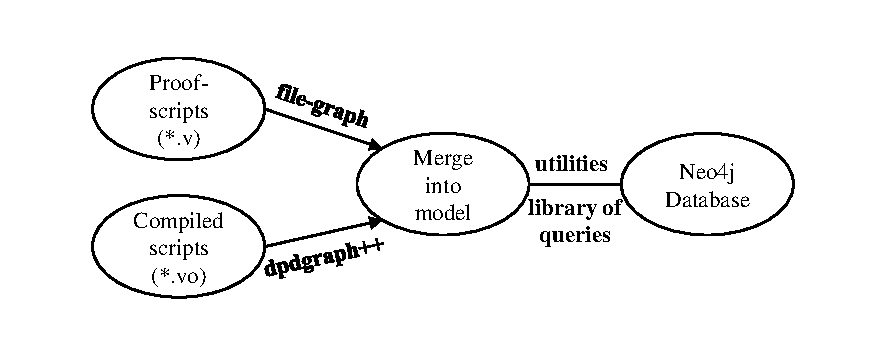
\includegraphics[width=\textwidth, page=1]{proposal/proposal-project-structure-diagram.pdf} 
\caption{System Components}\label{fig:structure}

\end{figure}


\section{Coq object-files to CSV}

This section of implementation corresponds to ``dpdgraph++'' on
Figure~\ref{fig:structure}: modelling the data contained in and the structure
of Coq object-files (\texttt{*.vo}) as comma-separated values (CSVs). The
initial model (inherited from the open-source ``dpdgraph'' tool) and subsequent
changes to it will be described.

\subsection{Modelling}

Initially, each edge was assigned a \emph{weight} representing the number of
(directed) uses of one node by another. Each node was assigned four
\emph{properties}: 

\begin{itemize}
  \item \emph{body}, a boolean representing whether a global declaration was
    either transparent or opaque;
  
  \item \emph{kind}, a ternary value representing whether a \emph{global
    reference} (a kernel side type for all references) was a reference to either
    the environment, an inductive type or a constructor of an inductive type;

  \item \emph{prop}, a boolean value representing whether a term is a \texttt{Prop}
    (a decidable, logical property about a program, as opposed to a
    general \texttt{Type});

  \item \emph{path}, a string value represent the module an object is in.
\end{itemize}

These properties were difficult to understand: they are not in the
vocabulary of a Coq programmer (e.g. \texttt{Definition}, \texttt{Inductive},
\texttt{Theorem}) and could not represent the richness of the
AST appropriately. It was not documented how to translate these constructs back
to familiar terms and thus, it quickly became clear that the these properties
needed to be replaced by more general and descriptive ones.

\subsubsection{Precise Kinds}

Apart from \emph{path}, all the properties were removed and replaced by two
\emph{labels}: labels are used to group  nodes into subsets; since a node can
belong to more than one subset, it can have more than one label assigned to it.
Implementation of this was straightforward: simply a matter of looking up and
expanding the abstract syntax tree starting from the type
\texttt{global\_reference}.

The two labels are \emph{kind} and \emph{subkind}.  A \emph{kind} is a string
which can take one of the following values, each directly corresponding to an
AST term: \textsf{module}, \textsf{class}, \textsf{type\_constructor},
\textsf{inductive\_type}, \textsf{definition}, \textsf{assumption} or
\textsf{proof}.

Optionally, some terms have \emph{subkinds}, for distinguishing different
constructs more precisely. For example, when writing Coq, there is no
\texttt{Proof} keyword; instead \texttt{Theorem}, \texttt{Lemma}, \texttt{Fact},
\texttt{Remark}, \texttt{Property}, \texttt{Proposition} and \texttt{Corollary}
all are \emph{synonyms} for proofs. Full details can be found in
Appendix~\ref{chapter:fullmodel}.

\subsubsection{Recursive Modules}

What remained from the initial model was the \emph{path} property. The issue
here was that an inherently \emph{hierarchical} structure (of inclusion) was
represented \emph{flatly} as a string attribute of a node. This made modules
second-class citizens, not subject to the same analyses and manipulations as
proof-objects, excluding the possibility of expressing \emph{module-level
dependencies} (as possible in the coqdep tool).

Implementing this feature was difficult; there were two major phases. Firstly,
the type of a node was exanded to include modules (using a variant datatype).
Finishing this was just a matter of locating and fixing the resulting
type-errors. This meant modules were in the model, but as a flat structure:
modules could be related to objects but not to other modules.

Thus, the second major phase was inferring and adding all the ``ancestors'' of
a module with the correct relationships (parent as source, child as
destination, repeatedly up to the root module). The initial attempt resulted in
stack-overflow for larger examples. A stack-trace did not highlight any point
of error so it was \emph{assumed} to be due to the na\"{i}ve, but easy-to-write
(and check) non-tail-recursive implementation. So, the code was rewritten in a
space-efficient tail-recursive manner (which allows for deeply nested module
hierarchies to be handled). Surprisingly, the problem persisted; further
investigation discovered the fault lay in the separate \texttt{dpd2} tool (the
details of which can be found in Subsection~\ref{subsec:translation}).

\subsubsection{Inductive Types and Constructors}

Now that the properties of the original dpdpgraph had been superseded by more
general and flexible alternatives, it was time to implement new features.  One
of the most obvious and frustrating omissions from the initial model was the
inability to relate an inductive type to to its constuctor(s). Expanding the 
AST term for type-constructors showed which type it constructed. However,

\subsubsection{Types}

Conducting a \emph{cognitive walkthrough} (detailed in
Chapter~\ref{chapter:evaluation}) spurred the addition of \emph{type
signatures} to the model. Type theory is central to a Coq user's work and being
able to include them in the model, would, along with kinds, subkinds and
modules, help towards meeting the modelling requirement~\ref{req:m1} of
including as much relevant data as possible. 

\emph{Getting} the type was unexpectedly straightfoward; following the
functions called when the Coq command \texttt{Check} \emph{<expression>} (for
printing the type of a given expression) led to the algorithm; all that was
left was converting the output to an OCaml string. It was \emph{using} the
output which was problematic. Newlines, quotation marks, and commas had to be
replaced by hash signs, single-quote marks and underscores respectively, so as
to not interfere with the \texttt{.dpd} and CSV encoding of data.


\subsubsection{Relationships}

Relationships were the most interesti
Intention, execution, problems (remember the stack overflow), solutions.

\begin{itemize}
  \item Tried and \emph{removed} x\_USED\_BY\_y
  \item USES
  \item CONTAINS
  \item CONSTRUCTED\_BY
  \item Emphasis on direction of arrow for exploration, importance of consistency
\end{itemize}

\subsection{Translation}
\label{subsec:translation}

\section{Coq source-files to CSV}
Intention, execution, problems, solutions.

Also, how it fit in with larger, open-source projects.

\subsection{Missing Information}

\subsection{Collection}
Explain Glob Files.

\subsection{Merging}

\section{CSV to Neo4j}
Intention, execution, problems, solutions.

Also, how it fit in with larger, open-source projects.

\subsection{Neo4j Import Tools}

\subsection{Impact of Changes to Model}
Trade-offs, execution.

\section{Query Library}
Intention, execution, problems, solutions.

Also, how it fit in with larger, open-source projects.

\subsection{APOC}

\subsection{Additions on top of APOC}

\subsection{igraph}

\subsubsection{Terminology}

\subsubsection{Betweenness Centrality}

\subsubsection{Closeness Centrality}

\subsubsection{PageRank}

\subsubsection{Community Detection}

\subsection{Visualisation}

\subsection{R Library}

\section{Project Related}
Modifying make files, testing, continuous-integration builds, editors

\section{Summary}
Features implemented, dead-ends and lessons learnt.
